\documentclass[12pt]{article}
\usepackage{amsmath, amssymb}
\usepackage{graphicx}
\usepackage{hyperref}
\usepackage{physics}
\usepackage{tikz}
\usetikzlibrary{calc}
\usepackage{amsthm}
\usepackage{epigraph}

\newtheorem*{principle}{Principle}

\usetikzlibrary{decorations.pathmorphing, arrows.meta, positioning}

\title{Time as a Dynamic Axis: An Operational Definition}
\author{Dickson Terrero}
\date{\today}

\begin{document}

\maketitle

\begin{quote}\itshape
Time is not a backdrop; it is the counted advance of processes, and the universe sets the count.
\end{quote}

\section*{Abstract}
We define time as a dynamic axis: the process–distance advanced by an admissible clock, converted into a coordinate by the universal constant \(c\). This operational definition, grounded in periodic physical transformations, recasts time not as a static backdrop but as an emergent coordinate from physical processes. We show that this definition leads naturally to the interpretation of time as a fourth dimension in relativistic spacetime.

\section{Overview and Roadmap}

\paragraph{Thesis at a glance.}
Time is a \emph{dynamic axis}: the process–distance advanced by an admissible clock, converted into a coordinate by the universal constant \(c\),
\[
\Delta t^{(B)}=\frac{\Delta s_B}{c}=N_B\,\tau_B,\qquad \Delta s_B:=N_B\,\lambda_B,\quad c=\frac{\lambda_B}{\tau_B}.
\]

\paragraph{Logical steps.}
\begin{enumerate}
  \item \textbf{Operational stance.} Choose any \emph{admissible} clock \(B\): a system with stable, reproducible cycles (\(\tau_B\)) and a calibrable scale \(\lambda_B\) satisfying \(c=\lambda_B/\tau_B\). Define its \emph{process–distance} \(\Delta s_B:=N_B\lambda_B\).
  \item \textbf{Duration (mechanism–independent).} For any process window, assign the duration \(\Delta t^{(B)}:=N_B\tau_B=\Delta s_B/c\). This is what clocks measure—no background time assumed.
  \item \textbf{Universality of \(c\).} Mild symmetry (relativity principle, spatial homogeneity/isotropy, reciprocity) implies a single conversion constant \(c\) for all admissible clocks; hence the duration is independent of the clock mechanism up to a fixed calibration \cite{BerziGorini1969,LevyLeblond1976,Mermin1984}.
  \item \textbf{Dynamic axis.} Because \(\Delta t^{(B)}\) is defined from a clock’s internal advance and is independent of spatial coordinates, it serves as an \emph{independent} coordinate axis. Kinematic quantities are relational, e.g.
  \[
  \mathbf v^{(B)}=\frac{d\mathbf x}{dt^{(B)}}=c\,\frac{d\mathbf x}{ds_B}.
  \]
  \item \textbf{4D representation (in inertial regions).} With invariant two-way \(c\), inertial charts are related by Lorentz transformations and admit a local \(3{+}1\) representation \((ct^{(B)},\mathbf x)\) with invariant
  \[
  c^2\,d\tau^2=c^2\,dt^{(B)2}-d\mathbf x^{\,2},
  \]
  i.e., a Lorentzian metric with signature \((+,-,-,-)\) \cite{Einstein1905,Rindler2006}.
  \item \textbf{Scope and tests.} The construction matches standard kinematics (e.g., time dilation via light clocks) and metrology (optical clocks), extends locally to curved spacetime via \(d\tau^2=(1/c^2)g_{\mu\nu}dx^\mu dx^\nu\), and remains purely operational \cite{Chou2010}.
\end{enumerate}

\paragraph{What we do \emph{not} assume.}
We do not assume a pre-existing global time, discreteness of time, or any special properties of light beyond the operational role of the invariant \(c\). For non-wave mechanisms, \(\lambda_B:=c/\nu_B\) is an \emph{associated} calibration scale.

\paragraph{How to read this note.}
The next section formalizes admissible clocks and calibration; the following section defines duration and states the relational principle; then we introduce “time as a dynamic axis” and its 4D Lorentzian representation. Short optional modules (radar synchronization, light-clock dilation, invariant interval, clock equivalence) and a quantum Ramsey appendix can be read independently.

\section{Admissible Clocks}

\paragraph{Definition.}
A \emph{clock} \(B\) is a system undergoing a reproducible periodic transformation
\(\mathcal{T}_{\mathrm{clock}}\) with a well-defined period \(\tau_B\) and an associated
wavelength \(\lambda_B\) satisfying
\begin{equation}
  c \;=\; \frac{\lambda_B}{\tau_B}
  \label{eq:core-equation}
\end{equation}
in the clock’s rest frame; i.e., the standard wave relation \(c=\lambda\,\nu\) with
\(\nu_B=1/\tau_B\).
\emph{For mechanisms that are not intrinsically wave-based,} \(\lambda_B:=c/\nu_B\) is an
\emph{associated} scale introduced for calibration; it need not correspond to a radiated wavelength.

\medskip
\noindent
Admissibility requires:
\begin{itemize}
    \item[(i)] \textbf{Periodicity}: stable, repeatable cycles;
    \item[(ii)] \textbf{Reproducibility under transport}: behavior remains consistent when transported between locations and inertial frames (as realized, e.g., by modern transportable and optical clocks \cite{Chou2010});
    \item[(iii)] \textbf{Calibrability}: can be referenced to the universal relation \eqref{eq:core-equation}.
\end{itemize}

\noindent\emph{Universality.} We assume that all admissible clocks share the same conversion constant \(c\) (derivable from the relativity principle, spatial isotropy, and reciprocity in fuller treatments) \cite{BerziGorini1969,LevyLeblond1976,Mermin1984}.

\paragraph{Terminology.}
A \emph{tick} denotes one completed cycle of an admissible clock. “Tick Theory” does \emph{not} assume time is fundamentally discrete; it is an operational counting procedure fully compatible with continuous limits.

\paragraph{Gloss (process–distance).}
For later use, define the clock’s \emph{process–distance} over a window by
\(\Delta s_B := N_B\,\lambda_B\); the operational duration relative to \(B\) is
\(\Delta t^{(B)}=\Delta s_B/c = N_B\,\tau_B\).


\section{Operational Definition of Duration}

\paragraph{Primary definition.}
Let \(N_B(\mathcal{T}_A)\) be the number of completed cycles of clock \(B\) during the process \(\mathcal{T}_A\).
The duration relative to \(B\) is
\begin{equation}
    \Delta t_A^{(B)} := N_B(\mathcal{T}_A)\,\tau_B,
    \label{eq:primary-duration}
\end{equation}
an explicitly operational stance (“time is what clocks measure”) in the spirit of Einstein’s 1905 construction of timekeeping and simultaneity \cite{Einstein1905}.

\paragraph{Wave-calibrated representation (optional).}
When a wave-based calibration is chosen for \(B\) (with wavelength \(\lambda_B\) satisfying \(c=\lambda_B/\tau_B\)), one may equivalently write
\begin{equation}
    \Delta t_A^{(B)} \;=\; \frac{N_B(\mathcal{T}_A)\,\lambda_B}{c}
    \;=\; \frac{\Delta s_B(\mathcal{T}_A)}{c},
    \label{eq:wave-duration}
\end{equation}
where \(\Delta s_B := N_B\,\lambda_B\) is the clock’s wave advance over the same window.
This is just the standard wave relation \(c=\lambda\nu\) with \(\nu=1/\tau_B\).\footnote{For non-radiating clocks (mechanical, orbital, or internal atomic transitions), the operational definition \eqref{eq:primary-duration} is sufficient and preferred.
Equation \eqref{eq:wave-duration} is a \emph{representation} convenient when comparing to spatial measures; introducing an associated \(\lambda_B=c/\nu_B\) is a metrological convention, not an additional physical claim.
Modern optical clock practice exemplifies the required stability and calibrability \cite{Chou2010}.}

\medskip
\noindent\emph{Note (associated wavelength).} For clocks that do not involve a propagating wave,
\(\lambda_B:=c/\nu_B\) is a \emph{defined associated scale} chosen so that \(c=\lambda_B/\tau_B\);
it need not represent a physical wavelength of the mechanism.

\medskip
\begin{principle}[Relational time]
Only relations between processes are measurable. Let \(B\) be any \emph{admissible} clock
that co-records a local process segment \(\mathcal T\) along a worldline (i.e., is co-located
on \(\mathcal T\)). Define
\[
T[\mathcal T]\;\equiv\;\Delta t^{(B)}(\mathcal T)
\;:=\; N_B(\mathcal T)\,\tau_B
\;=\; \frac{\Delta s_B(\mathcal T)}{c},
\qquad
\Delta s_B:=N_B\,\lambda_B .
\]
Then \(T\) is additive under concatenation and, by the universality assumption on \(c\)
(derivable from the relativity principle, spatial isotropy, and reciprocity \cite{BerziGorini1969,LevyLeblond1976,Mermin1984}),
mechanism-independent up to a fixed global scale (choice of units).
In inertial regions of Minkowski spacetime—using the standard two-way invariance of \(c\) and the clock hypothesis—the functional \(T[\mathcal T]\) coincides with proper time along that worldline \cite{Einstein1905,Rindler2006}.
\end{principle}

\newpage

\noindent Equation~\eqref{eq:wave-duration} restates this operationally: the duration of a
process is the process–distance advanced by the clock’s associated wave during that process,
divided by the universal conversion constant \(c\).
The unit choice is fixed by selecting a particular standard clock (e.g., SI second).

\medskip
\noindent\emph{Physical meaning.} Here \(\Delta s_B\) is the cumulative internal advance of the clock’s
periodic process. For wave clocks, one tick advances the phase by \(2\pi\) and the pattern by
one wavelength, so over \(N_B\) ticks \(\Delta s_B = N_B\lambda_B\). For non-wave (non-radiating)
clocks we introduce an \emph{associated} length per tick \(\lambda_B := c\,\tau_B = c/\nu_B\)
by metrological convention; this keeps \(\Delta t^{(B)}=\Delta s_B/c=N_B\tau_B\) uniform across
mechanisms. Note that \(\Delta s_B\) is neither a laboratory spatial displacement nor the
Minkowski interval.

\paragraph{Example (Non-wave clock: pendulum).}
Consider a simple pendulum: a non-radiating, mechanical clock. In a uniform gravitational
field and for small amplitudes, its period and frequency are
\[
\tau_B = 2\pi\sqrt{\frac{L}{g}}, 
\qquad 
\nu_B = \frac{1}{\tau_B}.
\]
Define its \emph{associated wavelength} by the metrological convention
\[
\lambda_B := \frac{c}{\nu_B} = c\,\tau_B,
\]
which is a defined scale (not a physical wavelength of emitted radiation). For \(N_B\) complete swings, the operational duration is
\[
\Delta t^{(B)} = N_B\,\tau_B
\;=\; \frac{N_B\,\lambda_B}{c}
\;=\; \frac{\Delta s_B}{c},
\qquad
\Delta s_B := N_B\,\lambda_B.
\]
Thus, the identity \(\Delta t^{(B)}=\Delta s_B/c\) holds for a non-wave mechanism as well,
illustrating \emph{mechanism-independence}. \emph{Admissibility caveat:} a simple pendulum
is only \emph{locally} admissible - \(\tau_B\) depends on \(g\) (and weakly on amplitude beyond
the small-angle regime), so reproducibility under transport fails when \(g\) changes; this is
why atomic clocks are preferred as portable standards.

\newpage

\section{Time as a Dynamic Axis}

\paragraph{Definition.}
Time is the \emph{process–distance} advanced by any admissible reference system (clock), converted into a coordinate by the universal constant \(c\) \cite{BerziGorini1969,LevyLeblond1976,Mermin1984}. For a clock \(B\) with period \(\tau_B\) and (possibly associated) wavelength \(\lambda_B\) calibrated by \(c=\lambda_B/\tau_B\), counting \(N_B\) ticks during a process gives
\begin{equation}
    \Delta t^{(B)} \;=\; N_B\,\tau_B \;=\; \frac{N_B\,\lambda_B}{c}
    \;=\; \frac{\Delta s_B}{c}, \qquad \Delta s_B := N_B\,\lambda_B,
\end{equation}
i.e., the wave-calibrated form of the operational relation \(c=\lambda\nu\) with \(\nu=1/\tau_B\) \cite{HechtOptics}. Thus, the time coordinate is generated by the advance of physical processes, rather than assumed as a static backdrop—and functions as a \emph{dynamic axis} independent of the spatial coordinates \cite{Einstein1905}.

\medskip
\noindent\emph{Consequence.}
With the relativity principle, spatial homogeneity/isotropy, reciprocity, and a universal \(c\), \(\Delta t^{(B)}=\Delta s_B/c\) serves as an independent coordinate, so events admit a local \(3{+}1\) chart \((ct^{(B)},\mathbf{x})\) with Lorentzian structure \cite{Minkowski1908,Rindler2006}.

\medskip
\noindent This dynamic axis is functionally distinct from spatial dimensions: it indexes the unfolding of causal processes and is represented by the time-like coordinate in a Lorentzian manifold.

\subsection*{No-Bridge Principle (Relational Reachability)}
\label{sec:no-bridge}

\begin{principle}[Principle (No-bridge, relational form)]
    Motion is not the enumeration of intermediate points but a \emph{correlation} between an
    evolving system \(A\) and an \emph{admissible} clock \(B\). If per tick of \(B\) the monitored
    quantity of \(A\) exhibits a strictly positive average advance, then a \emph{finite} tick
    budget reaches the target. No continuum needs to be ``crossed''.
\end{principle}

\paragraph{Reachability lemma (operational).}
Let \(x\) be the coordinate of interest for system \(A\). Suppose there exist \(\delta>0\) and
an integer \(m\ge 1\) such that for every consecutive block of \(m\) ticks of clock \(B\),
the net advance satisfies
\[
\Delta x_{\text{block}} \;\ge\; \delta.
\]
Then, starting from \(x=1\), one reaches \(x=2\) within at most
\[
N \;\le\; \Big\lceil \tfrac{2-1}{\delta} \Big\rceil\, m
\]
ticks of \(B\). In particular, the required number of ticks is finite.

\noindent\emph{Proof sketch.}
Concatenate blocks until the summed advance exceeds \(1\). Each block contributes at least
\(\delta\), so at most \(\lceil 1/\delta\rceil\) blocks are needed, i.e.\ at most
\(\lceil 1/\delta\rceil\,m\) ticks.

\paragraph{Corollary (dynamic-axis form).}
If along the evolution one has a bounded-away-from-zero relational drift
\[
\frac{dx}{dt^{(B)}} \;\ge\; v_{\min} \;>\; 0 \quad \text{for a.e.\ ticks},
\]
then the dynamic-axis duration to cover \(\Delta x\) obeys the finite bound
\[
\Delta t^{(B)} \;\le\; \frac{\Delta x}{v_{\min}}.
\]
Equivalently, in tick language: a positive average advance per tick implies a finite tick
count to reach the target.

\paragraph{Concrete mappings (physics, not enumeration).}
\begin{itemize}
  \item \textbf{Spaceflight (Earth \(\to\) Moon).} Let \(r\) be the Earth–craft range and
  \(B\) an onboard clock. If
  \(\frac{dr}{dt^{(B)}} \ge v_{\min} > 0\) almost everywhere, the tick budget to traverse
  \(\Delta r\) is bounded by
  \[
  \Delta t^{(B)} \;\le\; \frac{\Delta r}{v_{\min}}
  \quad\Rightarrow\quad
  N_B \;\le\; \frac{\Delta r}{v_{\min}\,\tau_B}.
  \]
  \item \textbf{Quantum evolution (two-level drive).} With Rabi frequency \(\Omega\),
  the phase advances as \(\phi=\Omega\,\Delta t^{(B)}\). A \(\pi\)-pulse reaches the target in
  \(\Delta t^{(B)}=\pi/\Omega\) (finite ticks \(N_B=\Omega\,\Delta t^{(B)}/2\pi=\tfrac12\)).
  \item \textbf{Relativistic worldlines.} Between two events,
  \[
  \Delta \tau \;=\; \frac{1}{c}\int \sqrt{\,c^2\,dt^{(B)2}-d\mathbf x^{\,2}\,}\,,
  \]
  which is finite for physical paths (bounded speeds, finite segments). Distinct paths yield
  different finite \(\Delta\tau\) without any ``enumeration'' of intermediate reals.
\end{itemize}

\paragraph{One-line takeaway.}
A strictly positive relational drift (per tick or per \(\Delta t^{(B)}\)) yields a \emph{finite}
tick budget to go from \(1\) to \(2\): motion is realized by \emph{relations} and finite counts,
not by visiting an infinity of intermediate points.

\section{Time as the Fourth Coordinate Dimension}

This framework shows that time behaves as a coordinate axis on equal mathematical footing with spatial dimensions. The process distance \(\Delta s_B\) is analogous to spatial displacements, and its conversion through \(c\) ensures compatibility with the relativistic spacetime structure \cite{Minkowski1908,Rindler2006}. The Lorentzian metric’s signature encodes the asymmetry between time and space, so this 'fourth dimension' is independent but not identical to the spatial axes \cite{Rindler2006}.

\begin{quote}
\textbf{Proposition.} \textit{Time functions as the fourth coordinate dimension in a relativistic manifold, generated operationally by periodic processes and scaled by the invariant conversion constant \(c\) \cite{Minkowski1908}.}
\end{quote}

\noindent Unlike space, however, time emerges from the evolution of processes and may retain a directional or causal asymmetry depending on the context (e.g., thermodynamics). Nonetheless, geometrically and operationally, it fulfills the role of a fourth dimension in Minkowski-type spacetimes \cite{Minkowski1908}.

\vspace{1.0em}

\begin{figure}[h!]
\centering
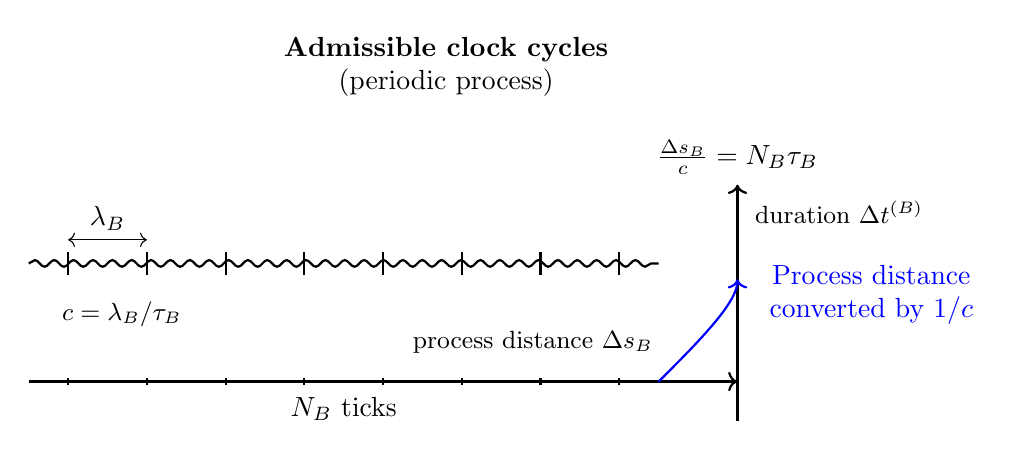
\begin{tikzpicture}[
    wave/.style={decorate, decoration={snake, amplitude=1.2pt, segment length=7pt}, thick},
    axis/.style={->, thick},
    tick/.style={thick}
]
% Clock wave
\draw[wave] (-4,1) -- (4,1);
% Tick marks on wave
\foreach \x in {-3.5, -2.5, -1.5, -0.5, 0.5, 1.5, 2.5, 3.5} {
    \draw[tick] (\x,0.85) -- (\x,1.15);
}
% Wavelength label
\draw[<->] (-3.5,1.3) -- (-2.5,1.3) node[midway, above] {\(\lambda_B\)};
% c = lambda/tau on the figure
\node[anchor=west] at (-3.7,0.35) {\small \(c=\lambda_B/\tau_B\)};
% Process distance axis (horizontal)
\draw[axis] (-4,-0.5) -- (5,-0.5);
\foreach \x in {-3.5, -2.5, -1.5, -0.5, 0.5, 1.5, 2.5, 3.5} {
    \draw[tick] (\x,-0.55) -- (\x,-0.45);
}
\node at (0,-0.85) {\(N_B\) ticks};
\node at (2.4,0) {\small process distance \(\Delta s_B\)};
% Time axis (vertical)
\draw[axis] (5,-1) -- (5,2.0) node[above] {\(\frac{\Delta s_B}{c} = N_B\tau_B\)};
\node[anchor=west] at (5.1,1.65) {\small duration \(\Delta t^{(B)}\)};
% Arrow from process distance to time axis
\draw[->, thick, blue] (4,-0.5) .. controls (4.5,0) and (5,0.5) .. (5,0.8);
% Clock label
\node[align=center] at (1.3,3.5) {\textbf{Admissible clock cycles}\\ (periodic process)}; 
% Conversion label
\node[align=center, blue] at (6.7,0.6) {\textcolor{blue}{Process distance}\\ \textcolor{blue}{converted by \(1/c\)}};
\end{tikzpicture}
\caption{An admissible clock defines time operationally. Counting \(N_B\) cycles gives a
process–distance \(\Delta s_B=N_B\lambda_B\); dividing by the universal conversion constant
\(c=\lambda_B/\tau_B\) yields the duration \(\Delta t^{(B)}=\Delta s_B/c=N_B\tau_B\).}
\end{figure}

\clearpage

\begin{figure}[htbp]
\centering
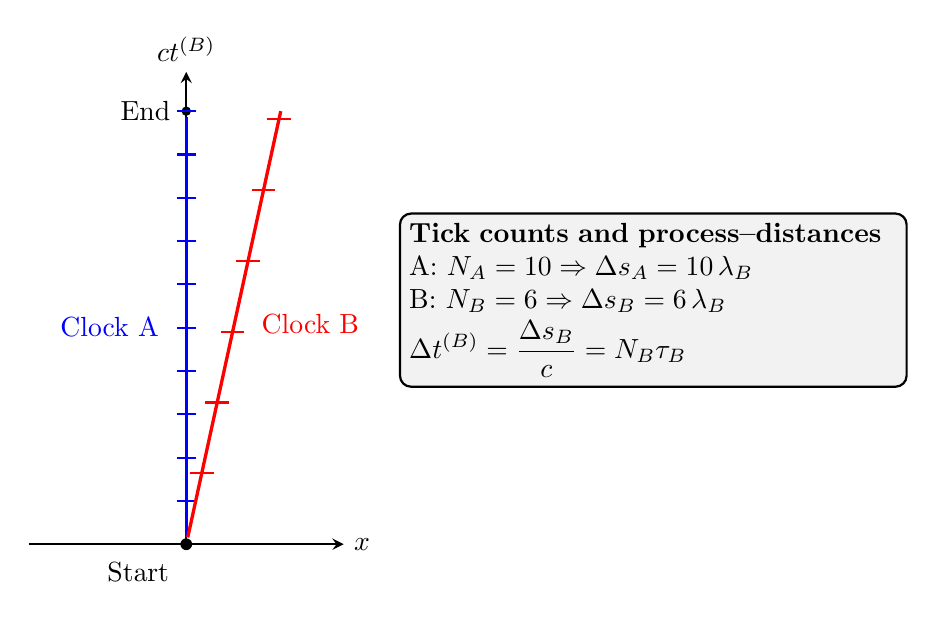
\begin{tikzpicture}[scale=1.0, thick, >=stealth,
  axis/.style={->, thick}, tick/.style={thick}]
% Axes
\draw[axis] (-2,0) -- (2,0) node[right] {$x$};
\draw[axis] (0,0) -- (0,6) node[above] {$ct^{(B)}$};

% Start/End events
\node[circle, fill=black, inner sep=1.5pt,
      label={[shift={(0,-0.35)}]left:Start}] (S) at (0,0) {};
\node[circle, fill=black, inner sep=1.2pt, label=left:{End}]   (E) at (0,5.5) {};

% Worldline A (rest): x=0
\draw[blue, very thick] (S) -- (E) node[midway, left=6pt, text=blue]{Clock A};

% Ticks for A: 10 evenly spaced along ct (proper ticks = coordinate ticks at rest)
\foreach \i in {1,...,10} {
  \draw[blue] (-0.12,0.55*\i) -- (0.12,0.55*\i);
}

% Worldline B (moving): slope v/c
\draw[red, very thick] (S) -- (1.2,5.5) node[midway, right=6pt, text=red]{Clock B};

% Ticks for B: fewer marks (6) over same coordinate time window
\foreach \y in {0.9, 1.8, 2.7, 3.6, 4.5, 5.4} {
  % place tick on the red line roughly at corresponding ct
  \pgfmathsetmacro{\x}{1.2*\y/5.5}
  \draw[red] (\x-0.15,\y) -- (\x+0.15,\y);
}

% Bubble with counts and process-distances
\node[draw, rounded corners, fill=gray!10, align=left, text width=6.2cm, anchor=west] at (2.7,3.1) {%
\textbf{Tick counts and process--distances}\\
A: $N_A=10 \Rightarrow \Delta s_A = 10\,\lambda_B$\\
B: $N_B=6 \Rightarrow \Delta s_B = 6\,\lambda_B$\\[2pt]
\(\displaystyle \Delta t^{(B)}=\frac{\Delta s_B}{c}=N_B\tau_B\)
};

\end{tikzpicture}
\caption{Two admissible clocks connecting the same start/end events. Clock A at rest (blue) accumulates
$N_A=10$ ticks; the moving clock B (red) accumulates $N_B=6$. Since \(\Delta t^{(B)}=\Delta s_B/c=N_B\tau_B\),
fewer ticks mean a smaller elapsed duration for B—an operational depiction of time dilation.}
\end{figure}

\section{Future Additions}

The present note is intentionally minimal: it defines duration operationally and frames
time as a dynamic axis generated by admissible clocks. To keep the scope lean while
signposting next steps, we list compact add-ons that can be included as brief modules
or appendices without altering the core construction. In all items below, time is treated
as an independent coordinate \(t^{(B)}\) derived from process–distance
(\(dt^{(B)}=ds_B/c\); over a window \(\Delta t^{(B)}=\Delta s_B/c\)) and paired with
spatial coordinates \(\mathbf{x}\). Here, \(ds_B\) denotes the differential
process–distance of the chosen admissible clock \(B\).

\paragraph{(A) Frame-level time via radar (Einstein synchronization).}
Using invariant two-way speed \(c\), define event coordinates on an inertial frame whose
\emph{spatial origin is co-located with the admissible clock \(B\)}. If a light signal is
sent at the frame’s clock reading \(t^{(B)}_{\mathrm{s}}\) and received back at
\(t^{(B)}_{\mathrm{r}}\), assign to the reflection event \(P\):
\[
t^{(B)}_E(P)=\tfrac{1}{2}\big(t^{(B)}_{\mathrm{s}}+t^{(B)}_{\mathrm{r}}\big),\qquad
x_E^{\parallel}(P)=\tfrac{c}{2}\big(t^{(B)}_{\mathrm{r}}-t^{(B)}_{\mathrm{s}}\big),
\]
with \(x_E^{\parallel}\) along the line of sight and transverse coordinates set by a rigid
orthogonal lattice (or two-baseline radar). This promotes local durations to a frame time
field \(t^{(B)}(\mathbf{x})\) without altering the dynamic-axis meaning of time \cite{Einstein1905}.

\paragraph{(B) Nontrivial kinematics from a light clock (time dilation).}
For a transverse light clock of arm length \(L\) moving at speed \(v\) relative to an
inertial frame with time \(t^{(B)}\), the path relation over one tick gives
\[
\Big(\tfrac{c\,\Delta t^{(B)}}{2}\Big)^2=\Big(\tfrac{v\,\Delta t^{(B)}}{2}\Big)^2+L^2
\;\Rightarrow\;
\Delta t^{(B)}=\gamma\,\Delta\tau_0,\qquad
\gamma=\frac{1}{\sqrt{1-v^2/c^2}},\quad
\]
\[
\Delta\tau_0=\frac{2L}{c}.
\]
Here \(\Delta\tau_0\) is the proper tick of the co-moving light clock, while
\(\Delta t^{(B)}\) is the coordinate duration recorded by the inertial frame’s time \(t^{(B)}\) \cite{Rindler2006}.

\paragraph{(C) Invariant interval and proper time (geometric tie-in).}
In inertial charts with time coordinate \(x^0=ct^{(B)}\), one has the quadratic invariant
\[
c^2(\Delta\tau)^2 \;=\; c^2\big(\Delta t^{(B)}\big)^2 - \|\Delta\mathbf{x}\|^2,
\]
consistent with metric signature \((+,-,-,-)\). Ideal admissible clocks measure \(\Delta\tau\)
along worldlines, specifying precisely how time is an independent axis with distinct signature
\cite{Rindler2006}.

\paragraph{(D) Clock equivalence on a worldline (formal lemma).}
For admissible clocks \(B,B'\) co-located on the same process segment \(\mathcal T\),
\[
T_{B'}(\mathcal T)=K_{BB'}\,T_B(\mathcal T),\qquad K_{BB'}>0,
\]
hence equality after a single calibration (\(K_{BB'}=1\)). This follows from additivity and
stability (optionally, an Archimedean/continuity property), with no additional physics assumptions
\cite{RovelliPartial}.

\paragraph{(E) Empirical anchors (metrology).}
Standard tests align with the construction: muon lifetime dilation, optical-clock
redshift in weak fields, and transport/synchronization comparisons \cite{Bailey1977,Chou2010,HafeleKeating1972a,Ashby2003}.
Clarify admissibility limits (clock hypothesis; environmental sensitivities of non-ideal mechanisms)

\paragraph{(F) Beyond inertial regions (brief note).}
Using coordinates \(x^0=ct^{(B)}\), proper time in curved spacetime generalizes via
\[
d\tau^2=\frac{1}{c^2}\,g_{\mu\nu}\,dx^\mu dx^\nu
\]
for signature \((+,-,-,-)\). Local inertial frames recover the inertial formulas with \(t^{(B)}\)
as the dynamic axis.

\paragraph{(G) Quantum interface (deferred).}
Phase accumulation and interferometric clocks couple directly to the dynamic axis,
e.g. \(\phi=\omega\,\Delta t^{(B)}\) with \(\omega=2\pi\nu_B\), while keeping the present note
purely operational and relativistic \cite{Ramsey1950}.

\section{Conclusion}
We have presented a minimal, operational construction of time: the duration of a process
is defined by counting ticks of an admissible clock, \(\Delta t^{(B)}=N_B\tau_B\), with an
equivalent wave-calibrated form \(\Delta t^{(B)}=\Delta s_B/c\) where \(\Delta s_B=N_B\lambda_B\)
and \(c=\lambda_B/\tau_B\). This identifies time as an \emph{dynamic axis} increase generated by
the advance of physical processes rather than as a static backdrop.

\medskip
\noindent
Within inertial regions, and adopting the standard two-way invariance of \(c\) \cite{Einstein1905},
this local construction supports the usual relativistic interpretation: time functions as an independent
coordinate on equal mathematical footing with space (with a distinct metric signature), enabling a
local \(3{+}1\) chart \((ct^{(B)},\mathbf{x})\). The “future additions” outline short, optional
modules, radar synchronization, light-clock dilation, the invariant interval, and a clock-equivalence statement of a lemma, which elevate the presentation from operational foundations to the familiar
Lorentz–Minkowski structure without altering the core thesis \cite{Rindler2006,Minkowski1908}.

\medskip
\noindent
The guiding perspective remains relational: only comparisons between processes are measurable,
and the universe provides the references. In this view, time is precisely the counted advance
of admissible processes, scaled by \(c\) \cite{RovelliPartial}.

\newpage

\appendix
\section*{Appendix: A Minimal Quantum Clock (Ramsey) and the Relation \(\phi=\omega_B\,\tau\)}

\subsection*{A. Model of an admissible quantum clock}
Consider a two–level system \(B\) with ground \(\ket{g}\), excited \(\ket{e}\), and rest–frame
Hamiltonian \(H_B=\tfrac{\hbar\omega_B}{2}\sigma_z\) (transition angular frequency \(\omega_B>0\)).
Let the clock co-move on a worldline \(\gamma\) with proper-time parameter \(\tau\). The free
evolution is
\[
U_0(\tau)=e^{-\,\tfrac{i}{\hbar}H_B\,\tau}
=\exp\!\Big(-\,\tfrac{i\omega_B\tau}{2}\sigma_z\Big),
\]
so any superposition accumulates a relative phase at rate \(\omega_B\) \emph{per unit proper time}
(\(\tau\)). \cite{Ramsey1950}

\subsection*{B. Ramsey sequence (operational readout of \(\tau\))}
Prepare \(\ket{g}\). Apply a resonant \(\pi/2\) pulse to create
\(\ket{\psi(0)}=\tfrac{1}{\sqrt{2}}(\ket{g}+\ket{e})\). Allow free evolution for a
co-moving proper duration \(\tau\), then apply a second \(\pi/2\) pulse with analysis
phase \(\theta\). The excited-state probability is
\[
P_e(\tau;\theta)=\tfrac{1}{2}\Big[1+C(\tau)\cos\!\big(\omega_B\tau+\phi_0-\theta\big)\Big],
\]
where \(\phi_0\) is a preparation phase and \(C(\tau)\in(0,1]\) the Ramsey contrast
(ideal clock: \(C=1\)). Thus the \emph{measured} phase advance is
\[
\phi_B(\tau)=\omega_B \tau+\phi_0 \quad\Rightarrow\quad
\boxed{\ \phi_B(\tau)-\phi_0=\omega_B\,\tau\ }\!,
\]
with maximal slope at \(\theta=\phi_0+\tfrac{\pi}{2}\). \cite{Ramsey1950}

\subsection*{C. Identification with the dynamic axis}
For a co-moving admissible clock, the operational time in the main text satisfies
\[
\Delta t^{(B)}=\frac{\Delta s_B}{c}=N_B\,\tau_B=\frac{\phi_B}{\omega_B},
\qquad \tau_B=\frac{2\pi}{\omega_B},\ \ N_B=\frac{\phi_B}{2\pi}.
\]
Hence, along the clock’s worldline \(\gamma\),
\[
\boxed{\ \Delta t^{(B)}=\tau\ } \qquad\text{and}\qquad
\boxed{\ \phi_B=\omega_B\,\Delta t^{(B)}=\omega_B\,\tau\ }.
\]
This realizes the “dynamic axis” in quantum terms: the process–distance is the accumulated
phase divided by \(\omega_B\), consistent with \(\Delta t^{(B)}=\Delta s_B/c\) using
\(\lambda_B=c/\nu_B\) and \(\omega_B=2\pi\nu_B\).

\subsection*{D. Relativistic tests (two clocks or two paths)}
Let two identical quantum clocks traverse worldlines \(\gamma_1,\gamma_2\) with proper times
\(\tau_1,\tau_2\). Their differential readout is
\[
\Delta\phi=\phi_1-\phi_2=\omega_B(\tau_1-\tau_2).
\]
In flat spacetime at constant speeds \(v_1,v_2\) relative to an inertial frame,
\(\tau=t^{(B)}\sqrt{1-v^2/c^2}=\gamma^{-1} t^{(B)}\), so
\[
\Delta\phi=\omega_B\,t^{(B)}\big(\gamma^{-1}_1-\gamma^{-1}_2\big),
\qquad \gamma=\frac{1}{\sqrt{1-v^2/c^2}}.
\]
In a weak gravitational field with potential \(\Phi\), the fractional redshift
\(\Delta f/f=\Delta\Phi/c^2\) gives
\[
\Delta\phi=\omega_B\!\int\!\frac{\Delta\Phi}{c^2}\,dt^{(B)},
\]
recovering gravitational time-dilation in the Ramsey phase. \cite{Will2014}

\subsection*{E. Measurement bounds (what limits \(\Delta t^{(B)}\) estimation?)}

\paragraph{Projection/shot noise (standard quantum limit).}
For \(M\) uncorrelated repetitions (or \(M\) atoms), the Fisher information for
\(P_e=\tfrac{1}{2}[1+C\cos\phi]\) at optimal bias (\(\phi\approx\pi/2\)) is \(F_1=C^2\),
so the Cram\'er–Rao bound is
\[
\Delta\phi \;\ge\; \frac{1}{C\sqrt{M}}
\quad\Rightarrow\quad
\Delta t^{(B)} \;\ge\; \frac{1}{\omega_B\,C\sqrt{M}}.
\]
Dephasing \(C(\tau)=e^{-\chi(\tau)}\) degrades precision accordingly.
\cite{Giovannetti2011}

\paragraph{Quantum speed limits (MT/ML).}
Writing \(\theta=\arccos|\braket{\psi(0)}{\psi(\tau)}|\), the evolution time obeys
\[
\tau \;\ge\; \max\!\left\{\frac{\hbar\,\theta}{2\,\Delta E},\;
\frac{\pi\hbar}{2\,(\langle H\rangle-E_0)}\right\},
\]
(Mandelstam–Tamm / Margolus–Levitin), which for free Ramsey precession is of order
\(1/\omega_B\). \cite{MT1945,ML1998}

\paragraph{Systematic limits.}
Finite interrogation time, dead time, reference laser noise, and environment sensitivity set practical
bounds; these affect \(C(\tau)\) and the total time uncertainty but do not alter
\(\phi=\omega_B\tau\).

\subsection*{F. Admissibility and mechanism–independence}
Any two admissible quantum clocks \(B,B'\) co-moving on the same worldline yield estimates related by
a fixed calibration factor:
\[
\hat t^{(B')}=K_{BB'}\,\hat t^{(B)},\qquad K_{BB'}=\frac{\omega_B}{\omega_{B'}}.
\]
After one calibration (\(K_{BB'}=1\)), both realize the same \(\tau\) within quantum
uncertainties. Thus the operational time of the main text coincides with proper time even
for intrinsically quantum clocks.

\subsection*{G. Summary}
A minimal Ramsey clock realizes the dynamic axis as follows: (i) free evolution imprints
\(\phi=\omega_B\tau\); (ii) the estimator \(\hat t^{(B)}=\hat\phi/\omega_B\) returns proper time
along the clock’s worldline; (iii) precision is bounded by projection noise and decoherence,
not by any mismatch between SR and QM. Differential phases between distinct worldlines measure
\(\Delta\tau\), directly connecting the operational definition of time to relativistic kinematics.

\newpage

\begin{thebibliography}{99}

% Relational / conceptual background (optional but aligned)
\bibitem{RovelliRQM}
C.~Rovelli.
\newblock Relational quantum mechanics.
\newblock \emph{Int. J. Theor. Phys.} \textbf{35}, 1637--1678 (1996).

\bibitem{RovelliPartial}
C.~Rovelli.
\newblock Partial observables.
\newblock \emph{Phys. Rev. D} \textbf{65}, 124013 (2002).

\bibitem{ConnesRovelliTTH}
A.~Connes and C.~Rovelli.
\newblock Von Neumann algebra automorphisms and time–thermodynamics relation in generally covariant quantum theories.
\newblock \emph{Class. Quantum Grav.} \textbf{11}, 2899--2918 (1994).

% Relativity without light / group-theoretic kinematics
\bibitem{BerziGorini1969}
V.~Berzi and V.~Gorini.
\newblock Reciprocity principle and the Lorentz transformations.
\newblock \emph{J. Math. Phys.} \textbf{10}, 1518--1524 (1969).

\bibitem{LevyLeblond1976}
J.-M. L\'evy-Leblond.
\newblock One more derivation of the Lorentz transformation.
\newblock \emph{Am. J. Phys.} \textbf{44}, 271--277 (1976).

\bibitem{Mermin1984}
N.~D. Mermin.
\newblock Relativity without light.
\newblock \emph{Am. J. Phys.} \textbf{52}, 119--124 (1984).

% Synchronization / spacetime geometry classics
\bibitem{Einstein1905}
A.~Einstein.
\newblock Zur Elektrodynamik bewegter K\"orper.
\newblock \emph{Ann. Phys.} \textbf{17}, 891--921 (1905).

\bibitem{Minkowski1908}
H.~Minkowski.
\newblock Space and Time (1908). English translation in \emph{The Principle of
Relativity} (Einstein, Lorentz, Weyl, Minkowski), Dover, 1952.

\bibitem{Minkowski1909}
H.~Minkowski.
\newblock Raum und Zeit.
\newblock \emph{Phys. Z.} \textbf{10}, 75--88 (1909).

% Empirical anchors / metrology
\bibitem{Ashby2003}
N.~Ashby.
\newblock Relativity in the Global Positioning System.
\newblock \emph{Living Rev. Relativ.} \textbf{6}, 1 (2003).

\bibitem{HafeleKeating1972a}
J.~C. Hafele and R.~E. Keating.
\newblock Around-the-World Atomic Clocks: Predicted Relativistic Time Gains.
\newblock \emph{Science} \textbf{177}, 166--168 (1972).

\bibitem{HafeleKeating1972b}
J.~C. Hafele and R.~E. Keating.
\newblock Around-the-World Atomic Clocks: Observed Relativistic Time Gains.
\newblock \emph{Science} \textbf{177}, 168--170 (1972).

\bibitem{Bailey1977}
J.~Bailey \emph{et al.}
\newblock Measurements of relativistic time dilatation for positive and negative muons in a circular orbit.
\newblock \emph{Nature} \textbf{268}, 301--305 (1977).

\bibitem{PoundRebka1960}
R.~V. Pound and G.~A. Rebka, Jr.
\newblock Apparent Weight of Photons.
\newblock \emph{Phys. Rev. Lett.} \textbf{4}, 337--341 (1960).

\bibitem{Chou2010}
C.~W. Chou, D.~B. Hume, T.~Rosenband, and D.~J. Wineland.
\newblock Optical clocks and relativity.
\newblock \emph{Science} \textbf{329}, 1630--1633 (2010).

% Textbook anchor for clock hypothesis / SR basics
\bibitem{Rindler2006}
W.~Rindler.
\newblock \emph{Relativity: Special, General, and Cosmological}, 2nd ed.
\newblock Oxford University Press, 2006.

\bibitem{HechtOptics}
E.~Hecht, \emph{Optics}, 4th ed. (Addison Wesley, San Francisco, 2002).


\bibitem{Ramsey1950}
N.~F. Ramsey.
\newblock A molecular beam resonance method with separated oscillating fields.
\newblock \emph{Phys. Rev.} \textbf{78}:695--699, 1950.

\bibitem{Giovannetti2011}
V.~Giovannetti, S.~Lloyd, and L.~Maccone.
\newblock Advances in quantum metrology.
\newblock \emph{Nature Photonics} \textbf{5}:222--229, 2011.

\bibitem{MT1945}
L.~Mandelstam and I.~Tamm.
\newblock The uncertainty relation between energy and time in non-relativistic quantum mechanics.
\newblock \emph{J. Phys. (USSR)} \textbf{9}:249--254, 1945.

\bibitem{ML1998}
N.~Margolus and L.~B. Levitin.
\newblock The maximum speed of dynamical evolution.
\newblock \emph{Physica D} \textbf{120}:188--195, 1998.

\bibitem{Will2014}
C.~M. Will.
\newblock The confrontation between general relativity and experiment.
\newblock \emph{Living Reviews in Relativity} \textbf{17}:4, 2014.

\end{thebibliography}

\end{document}
